\chapter{Introduction}\label{ch-introduction}
\thispagestyle{headings}
\markboth{Chapter \ref{ch-introduction}: Introduction}{Chapter \ref{ch-introduction}: Introduction}

%The purpose of this chapter is to introduce the main concepts and results necessary for
%a more formal treatment of the prediction problem.
%Section \ref{sc-intro-qoi} presents a first mathematical model of a system, as well as the applicability of Bayes' theorem to our prediction problem.
%The chapter finishes with the presentation of a more detailed model of a system in Section \ref{sc-intro-detail}.

Other docs: \cite{PrSc09} and html.

\section{Key Statisitcal Concepts}

\begin{figure}[h!]
\centerline{
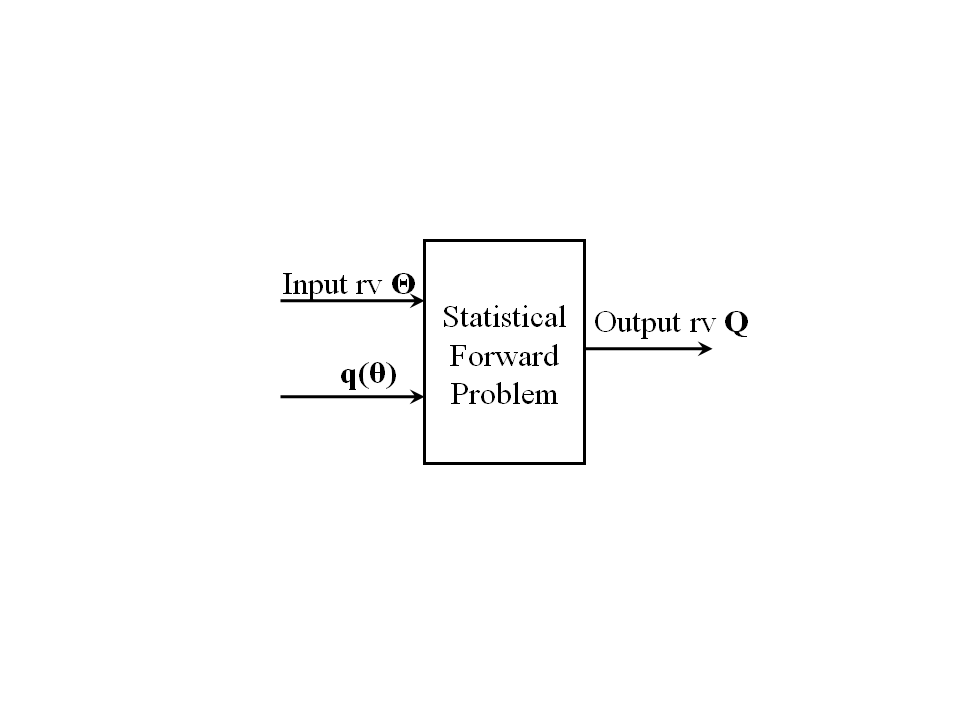
\includegraphics[scale=0.45,clip=true,viewport=1.0in 2.5in 10.0in 5.5in]{figs/queso_paper1_09.eps}
}
\caption{
The representation of a statistical forward problem.
$\boldsymbol{\Theta}$ denotes a random variable related to parameters,
$\boldsymbol{\theta}$ denotes a realization of $\boldsymbol{\Theta}$ and
$\mathbf{Q}$ denotes a random variable related to quantities of interest.
}
\label{fig-sfp-queso}
\end{figure}

\begin{figure}[h!]
\centerline{
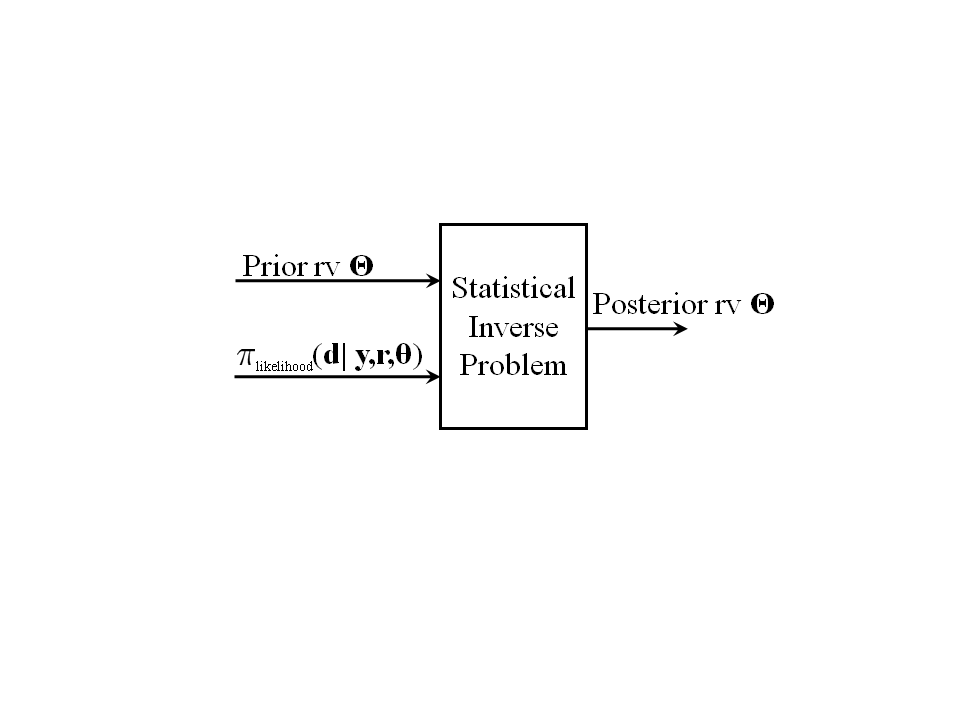
\includegraphics[scale=0.45,clip=true,viewport=1.0in 3.0in 10.0in 5.5in]{figs/queso_paper1_10.eps}
}
\caption{
The representation of a statistical inverse problem.
$\boldsymbol{\Theta}$ denotes a random variable related to parameters,
$\boldsymbol{\theta}$ denotes a realization of $\boldsymbol{\Theta}$ and
$\mathbf{r}$ denotes model equations,
$\mathbf{y}$ denotes some model output data and
$\mathbf{d}$ denotes experimental data.
}
\label{fig-sip-queso}
\end{figure}

\section{The Software Stack of an Application Using QUESO}

\begin{figure}[h!]
\centerline{
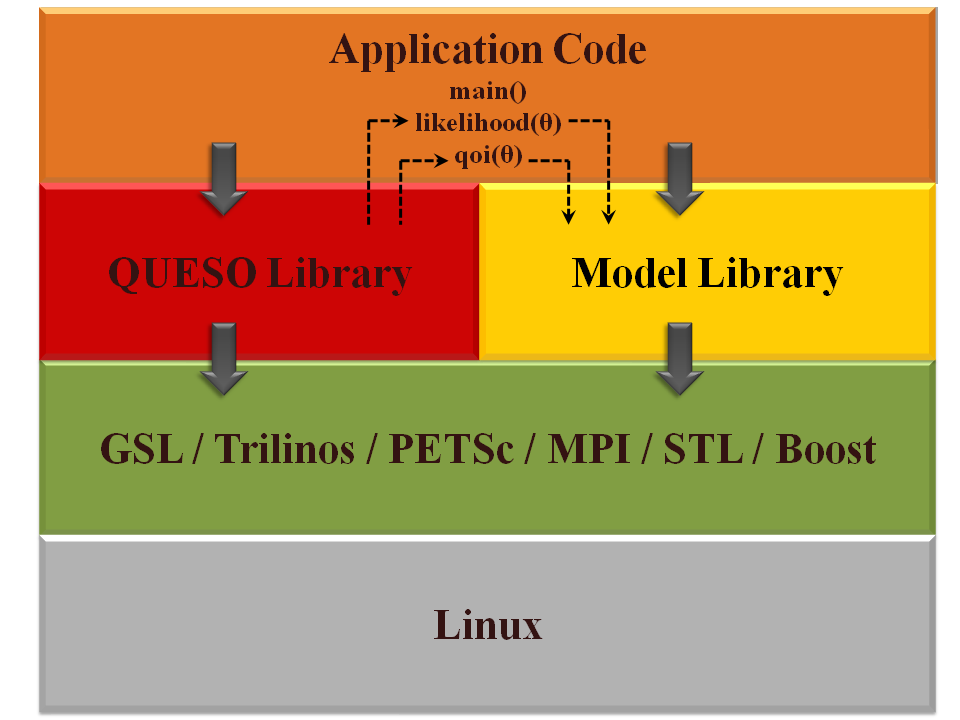
\includegraphics[scale=0.50,clip=true]{figs/queso_paper1_03.eps}
}
\caption{
Overview of the software stack of a typical application that uses QUESO.
Algorithms in the QUESO library require the supply
of a likelihood routine $\pi_{\text{like}}:\mathbb{R}^n\rightarrow\mathbb{R}_+$ for statistical inverse problems and 
of a qoi routine $\mathbf{q}:\mathbb{R}^n\rightarrow\mathbb{R}^m$ for statistical forward problems. These routines
exist at the application level and provide the necessary bridge between the statistical algorithms in QUESO,
model knowledge in the model library and scenario and experimental data in the disk space.
Concepts are further detailed in Chapter \ref{ch-introduction}.
}
\label{fig-sw-stack}
\end{figure}

\subsection{A QUESO Environment}

\subsection{Using Other C++ Classes in the Library}

\subsection{Input and Output Files}

